\documentclass[12pt, french]{article}

\usepackage[utf8]{inputenc}
\usepackage[T1]{fontenc}
\usepackage{titlesec}
\usepackage{graphicx}
%\newcommand{\sectionbreak}{\clearpage}
\usepackage[table]{xcolor}
\usepackage[left=3cm,right=3cm,top=2cm,bottom=2cm]{geometry}

\definecolor{darkgreen}{rgb}{0.0, 0.2, 0.13}

\usepackage{listings}
\lstset{
	language=[Sharp]C,
	backgroundcolor=\color{black!5},
	basicstyle=\footnotesize,
	breaklines=true,
	postbreak=\mbox{\textcolor{red}{$\hookrightarrow$}\space},
	frame=tb,
	tabsize=4,
	showstringspaces=false,
	numbers=left,
	commentstyle=\color{red},
	keywordstyle=\color{blue},
	stringstyle=\color{darkgreen}
	}

\title{\Huge{ Vision, Réalité virtuelle et augmentée\\~\\Compte rendu TP3 : \\Unity}}
\author{Luc Senecal}
\date{\today}

\begin{document}
\maketitle
\newpage

\section{Transitions}

Dans l'image suivante, on peut voir la transition en cours. Certains arbres sont encore discernable.

\begin{figure}[h]
\centering
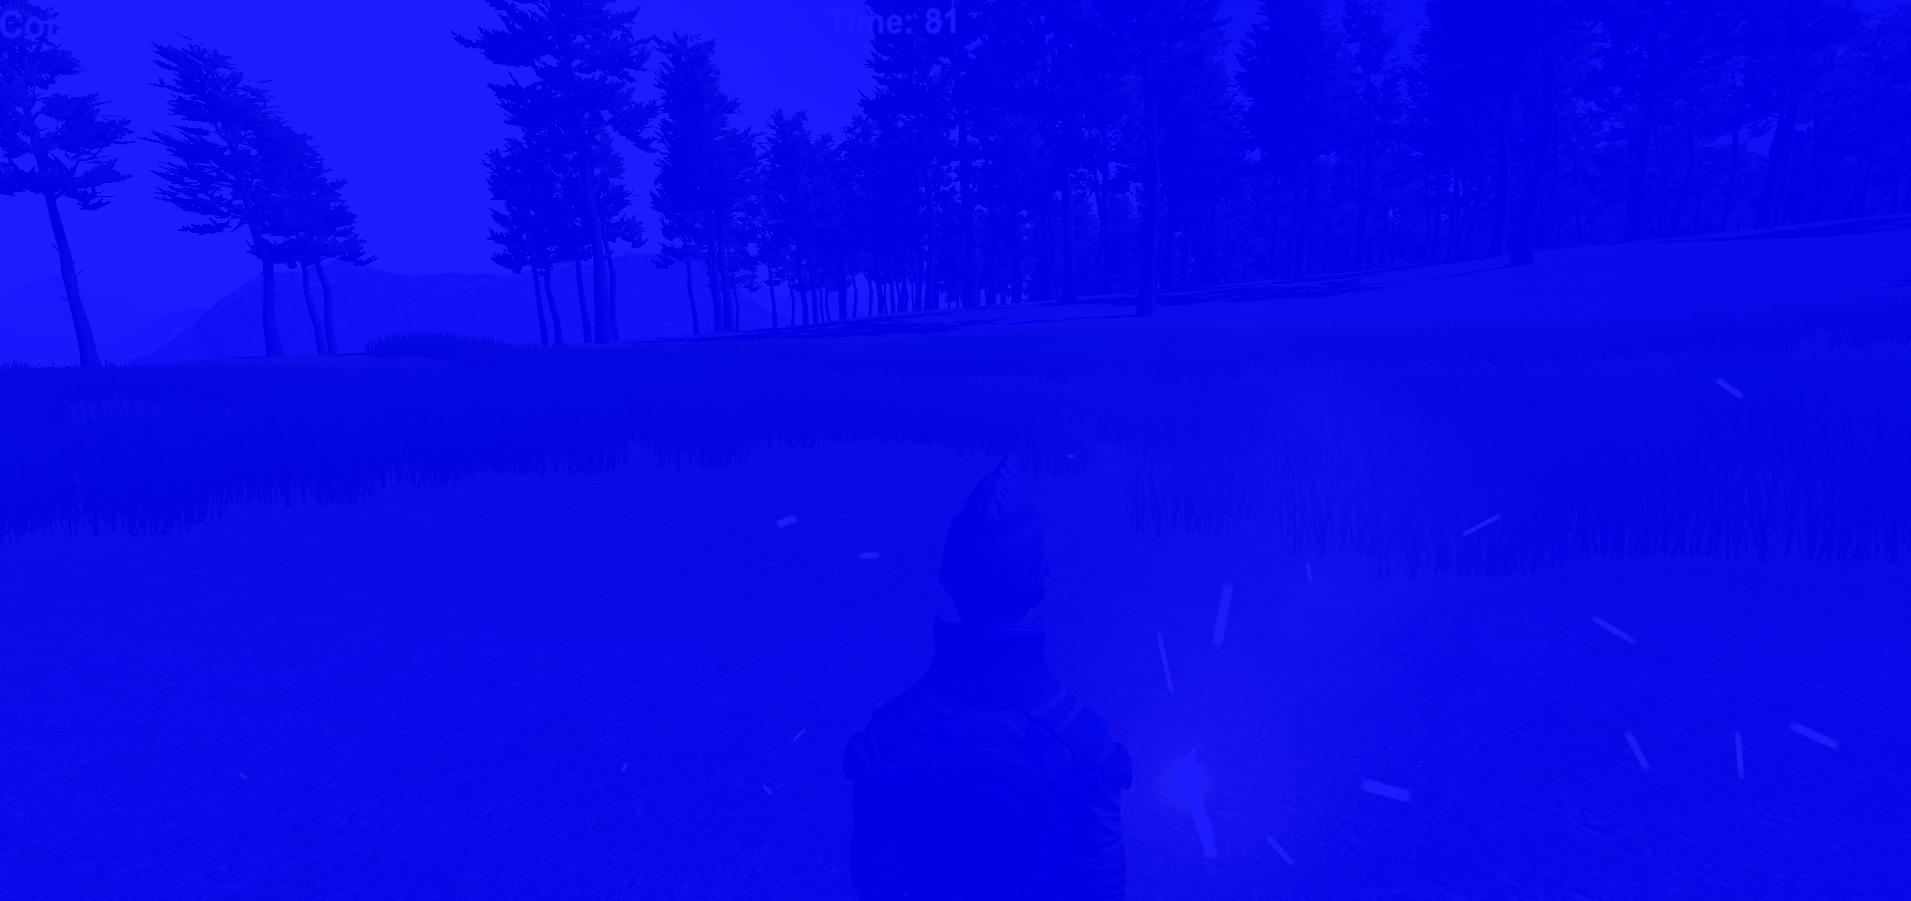
\includegraphics[width = \linewidth]{transition}
\caption{Moment de la transition}
\end{figure}

\begin{figure}[h]
\centering
\includegraphics[width = 0.6\linewidth]{animator}
\caption{Animator}
\end{figure}

\clearpage
\section{Interface VR}

\begin{figure}[h]
\centering
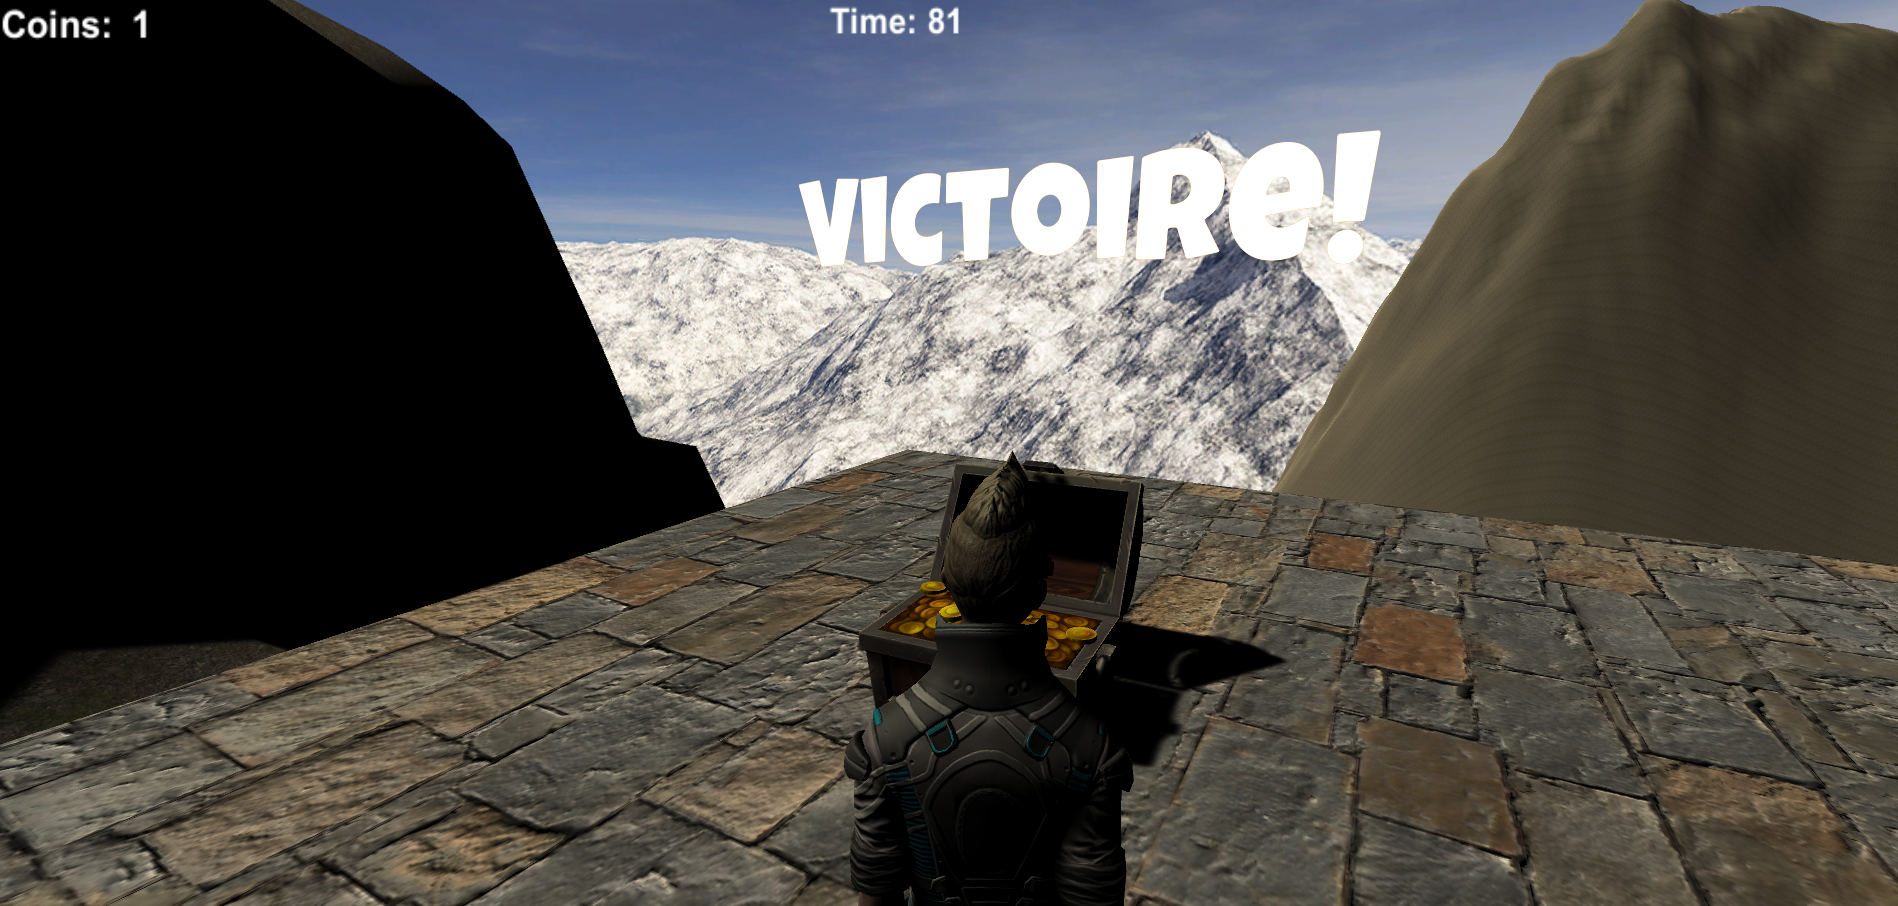
\includegraphics[width = \linewidth]{interface}
\caption{UI 3D}
\end{figure}

\section{Labyrinthe}

J'ai utilisé la texture pour poser les murs, mais je l'ai remplacée ensuite. J'ai ajouté une seconde lumière directionnelle pour éviter des murs noirs.

\begin{figure}[h]
\centering
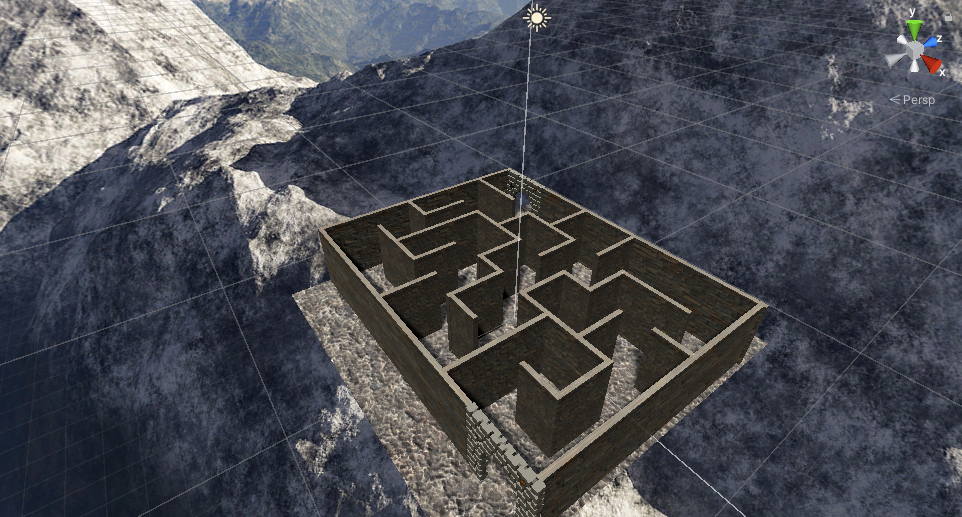
\includegraphics[width = 0.9\linewidth]{laby}
\caption{Labyrinthe}
\end{figure}

\clearpage
\section{De la continuité du temps}

On peut voir sur l'image que le timer continue après être rentré dans le niveau du labyrinthe.

\begin{figure}[h]
\centering
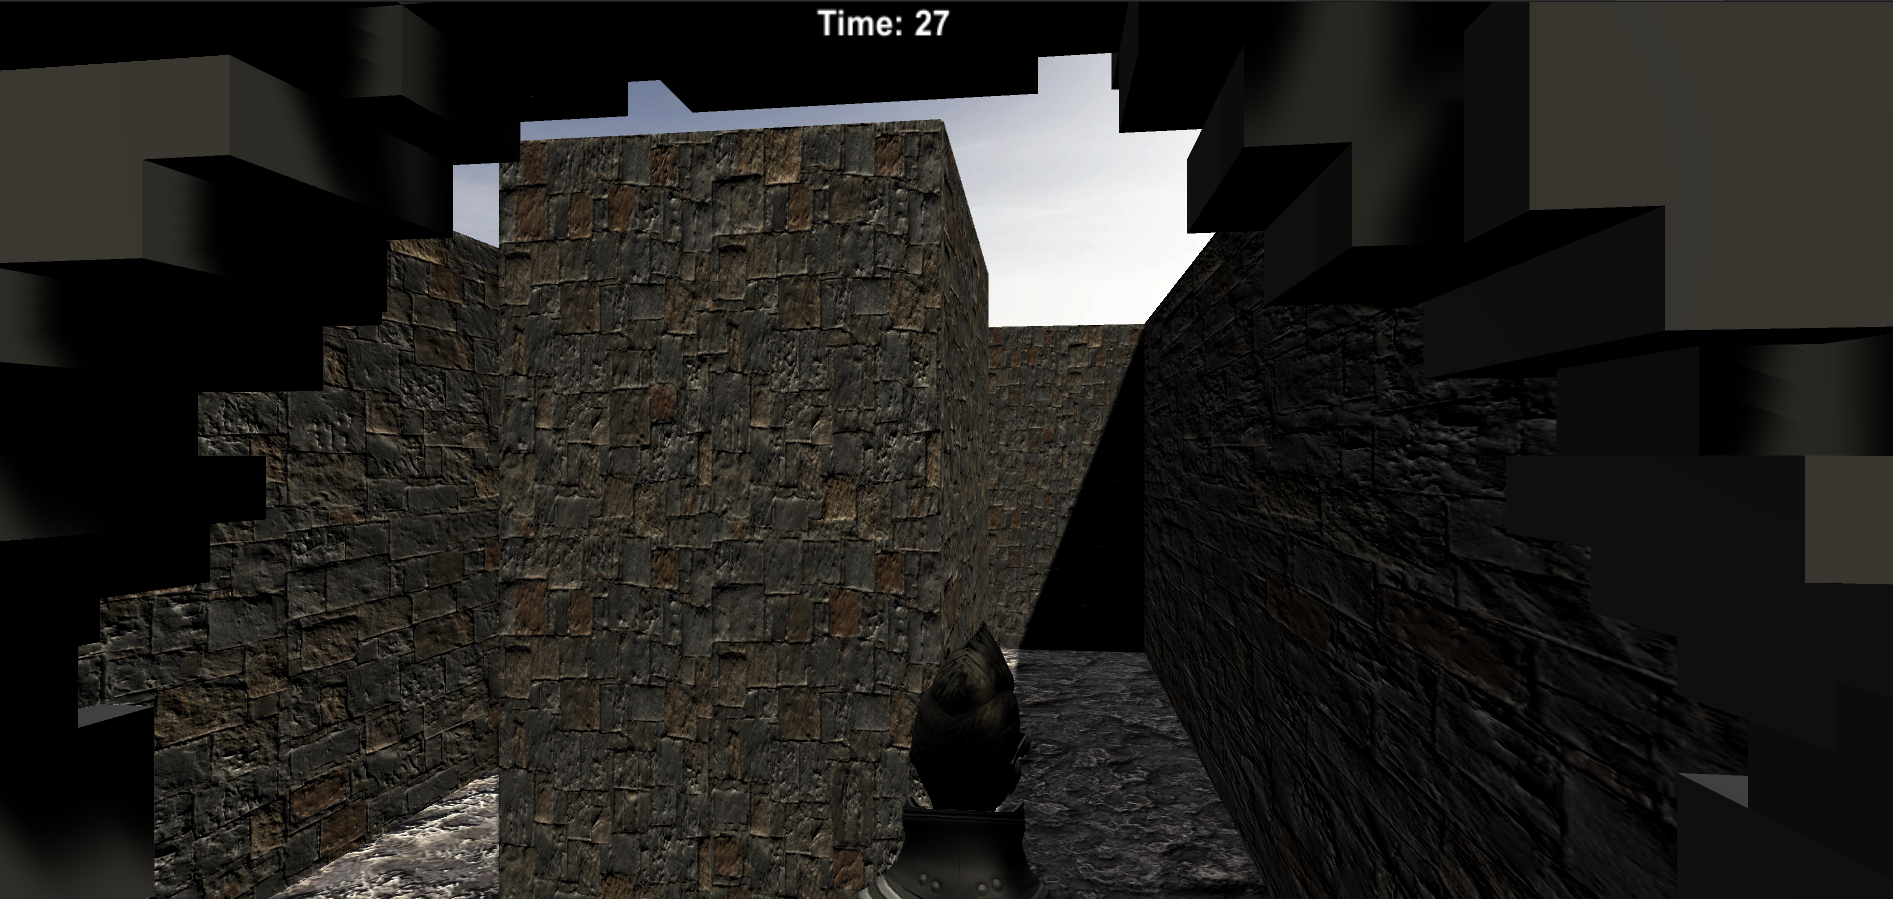
\includegraphics[width = \linewidth]{timer}
\caption{Le timer continue d'une scène à l'autre}
\end{figure}

\section{Fungus}

\begin{figure}[h]
\centering
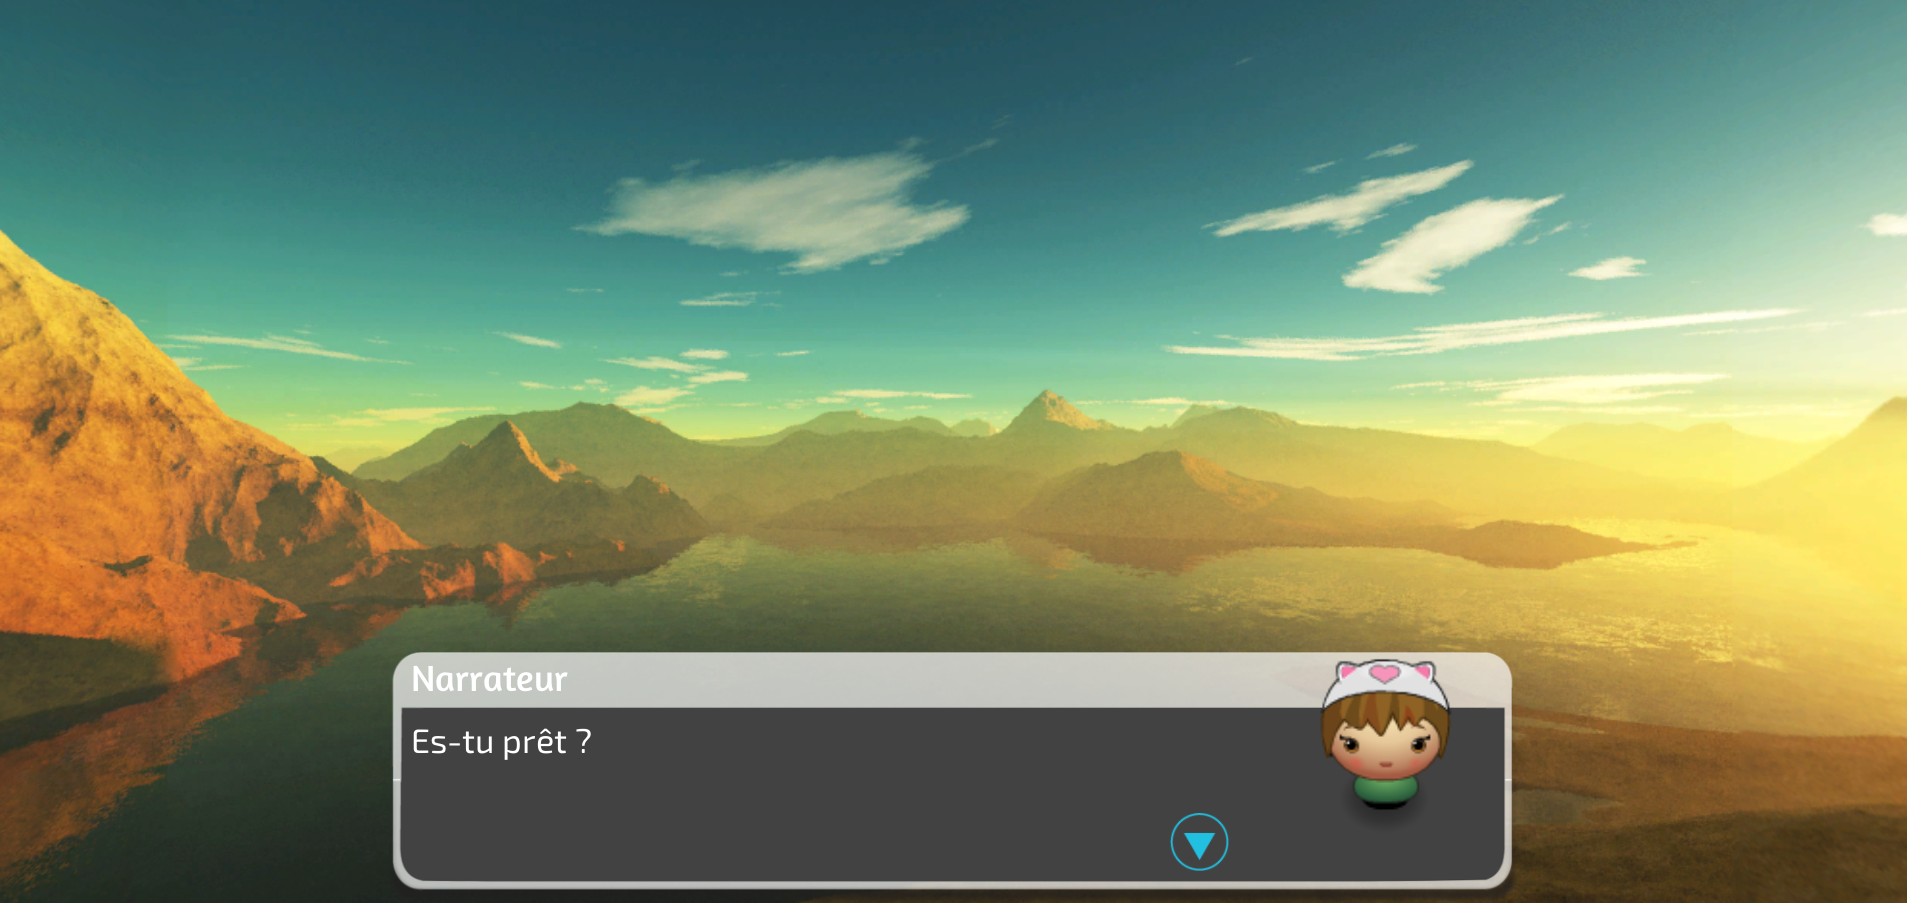
\includegraphics[width = \linewidth]{narrateur}
\caption{Introduction par le narrateur}
\end{figure}

\clearpage
\section{Les plateformes}

\begin{figure}[h]
\centering
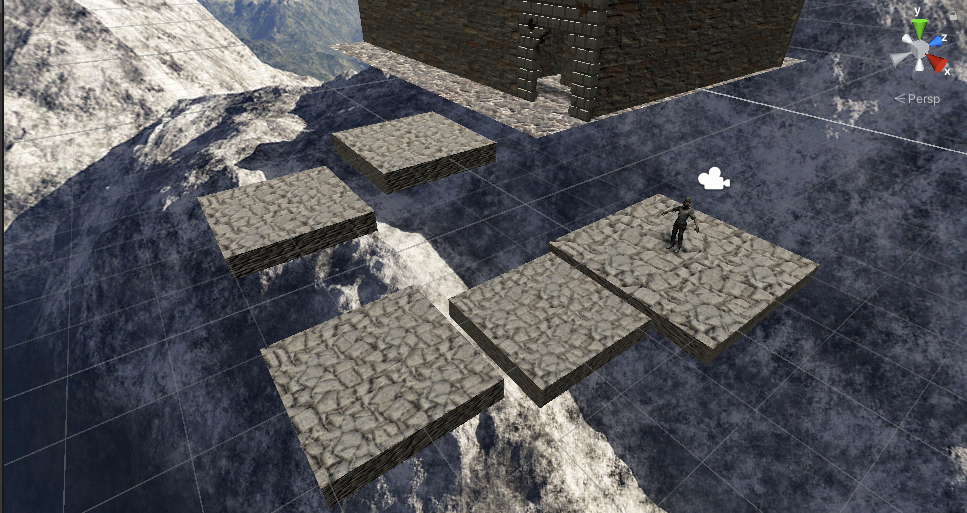
\includegraphics[width = \linewidth]{plateforme}
\caption{Jeu de plateforme pour le joueur}
\end{figure}

\section{Conclusion}
Tout s'est déroulé sans accroc.
\end{document}